\chapter{Implementace}
V této kapitole bude obsažen popis implementace návrhu z předchozích kapitol. Budou zde do detailu rozebrány jednotlivé části implementace a popsány problémy, které se vyskytly během vývoje.

\section{Komponenty frontendové aplikace}
V následující sekci budou popsány jednotlivé funkční komponenty, které byly implementovány v rámci frontendové části této práce. Všechny byly implementovány tak, aby komunikovaly s databází pomocí API.

\subsection{Přihlašování}
Přihlašování je první komponenta, která je uživateli po navštívení stránky zobrazena. Jedná se o obyčejný formulář se dvěma poli, kde uživatel zadá své licenční číslo a heslo. Po odeslání formuláře se data odešlou na server, kde se porovnají s daty v databázi. Pokud je vše v pořádku, tak se z API vrátí odpověď s tokenem a identifikátorem licence a obě tyto informace se uloží do relace. Token se dále používá pro autorizaci dotazů. Následně je uživatel přesměrován na další komponentu. V případě, že je příhlášení chybné, je uživateli zobrazena chybová hláška. Jedná se o jednoduchou komponentu, která nevyžaduje žádné složité operace, tudíž ani její implementace nebyla nijak složitá.

\subsection{Výběr dobrodružství}
Tato komponenta následuje hned po přihlášení. Zde si může uživatel prohlédnout, vybrat, či vytvořit takzvané dobrodružství [\ref{sec:dobrodruzstvi}]. Každé z nich má vlastní kartu, která obsahuje název, popis a výčet zdrojů, které mají hráči dostupné. Uživatel si může vybrat dobrodružství, které chce hrát, a následně je přesměrován na další komponentu. Pokud si žádné nevybere, může si vytvořit nové. Vytvoření nového dobrodružství je možné pouze v případě, že jich na dané licenci existuje méně než osm, což by mělo být dostatečné množství. Zároveň je zde možnost dobrodružství smazat, či upravit jeho název a popis. Jedná se jen o málo složitější komponentu, která vyžaduje komunikaci s API na více místech.

\subsection{Vytvoření postav}
Pokud si uživatel vytvoří nové dobrodružtví, či si vybere nějaké, ve kterém prozatím nejsou žádné postavy, je přesměrován na tuto komponentu. Zde si může vytvořit až šest postav, které budou v daném dobrodružtví učinkovat. Každé z postav hráč přiřadí jméno, jméno hráče a dále vybere její rasu a povolání. Ty společně určují hráčovy statistiky, jako body životů, obranu a iniciativu. Každá rasa a povolání má svůj vlastní obrázek, který ji představuje. Po vybrání obou možností se také zobrazí finální obrázek postavy, který odpovídá kombinaci zvolených možností. Zároveň se při změně jedné z nich změní jak obrázek, tak i výpis statistik.

\begin{figure}[htbp]
  \centering
  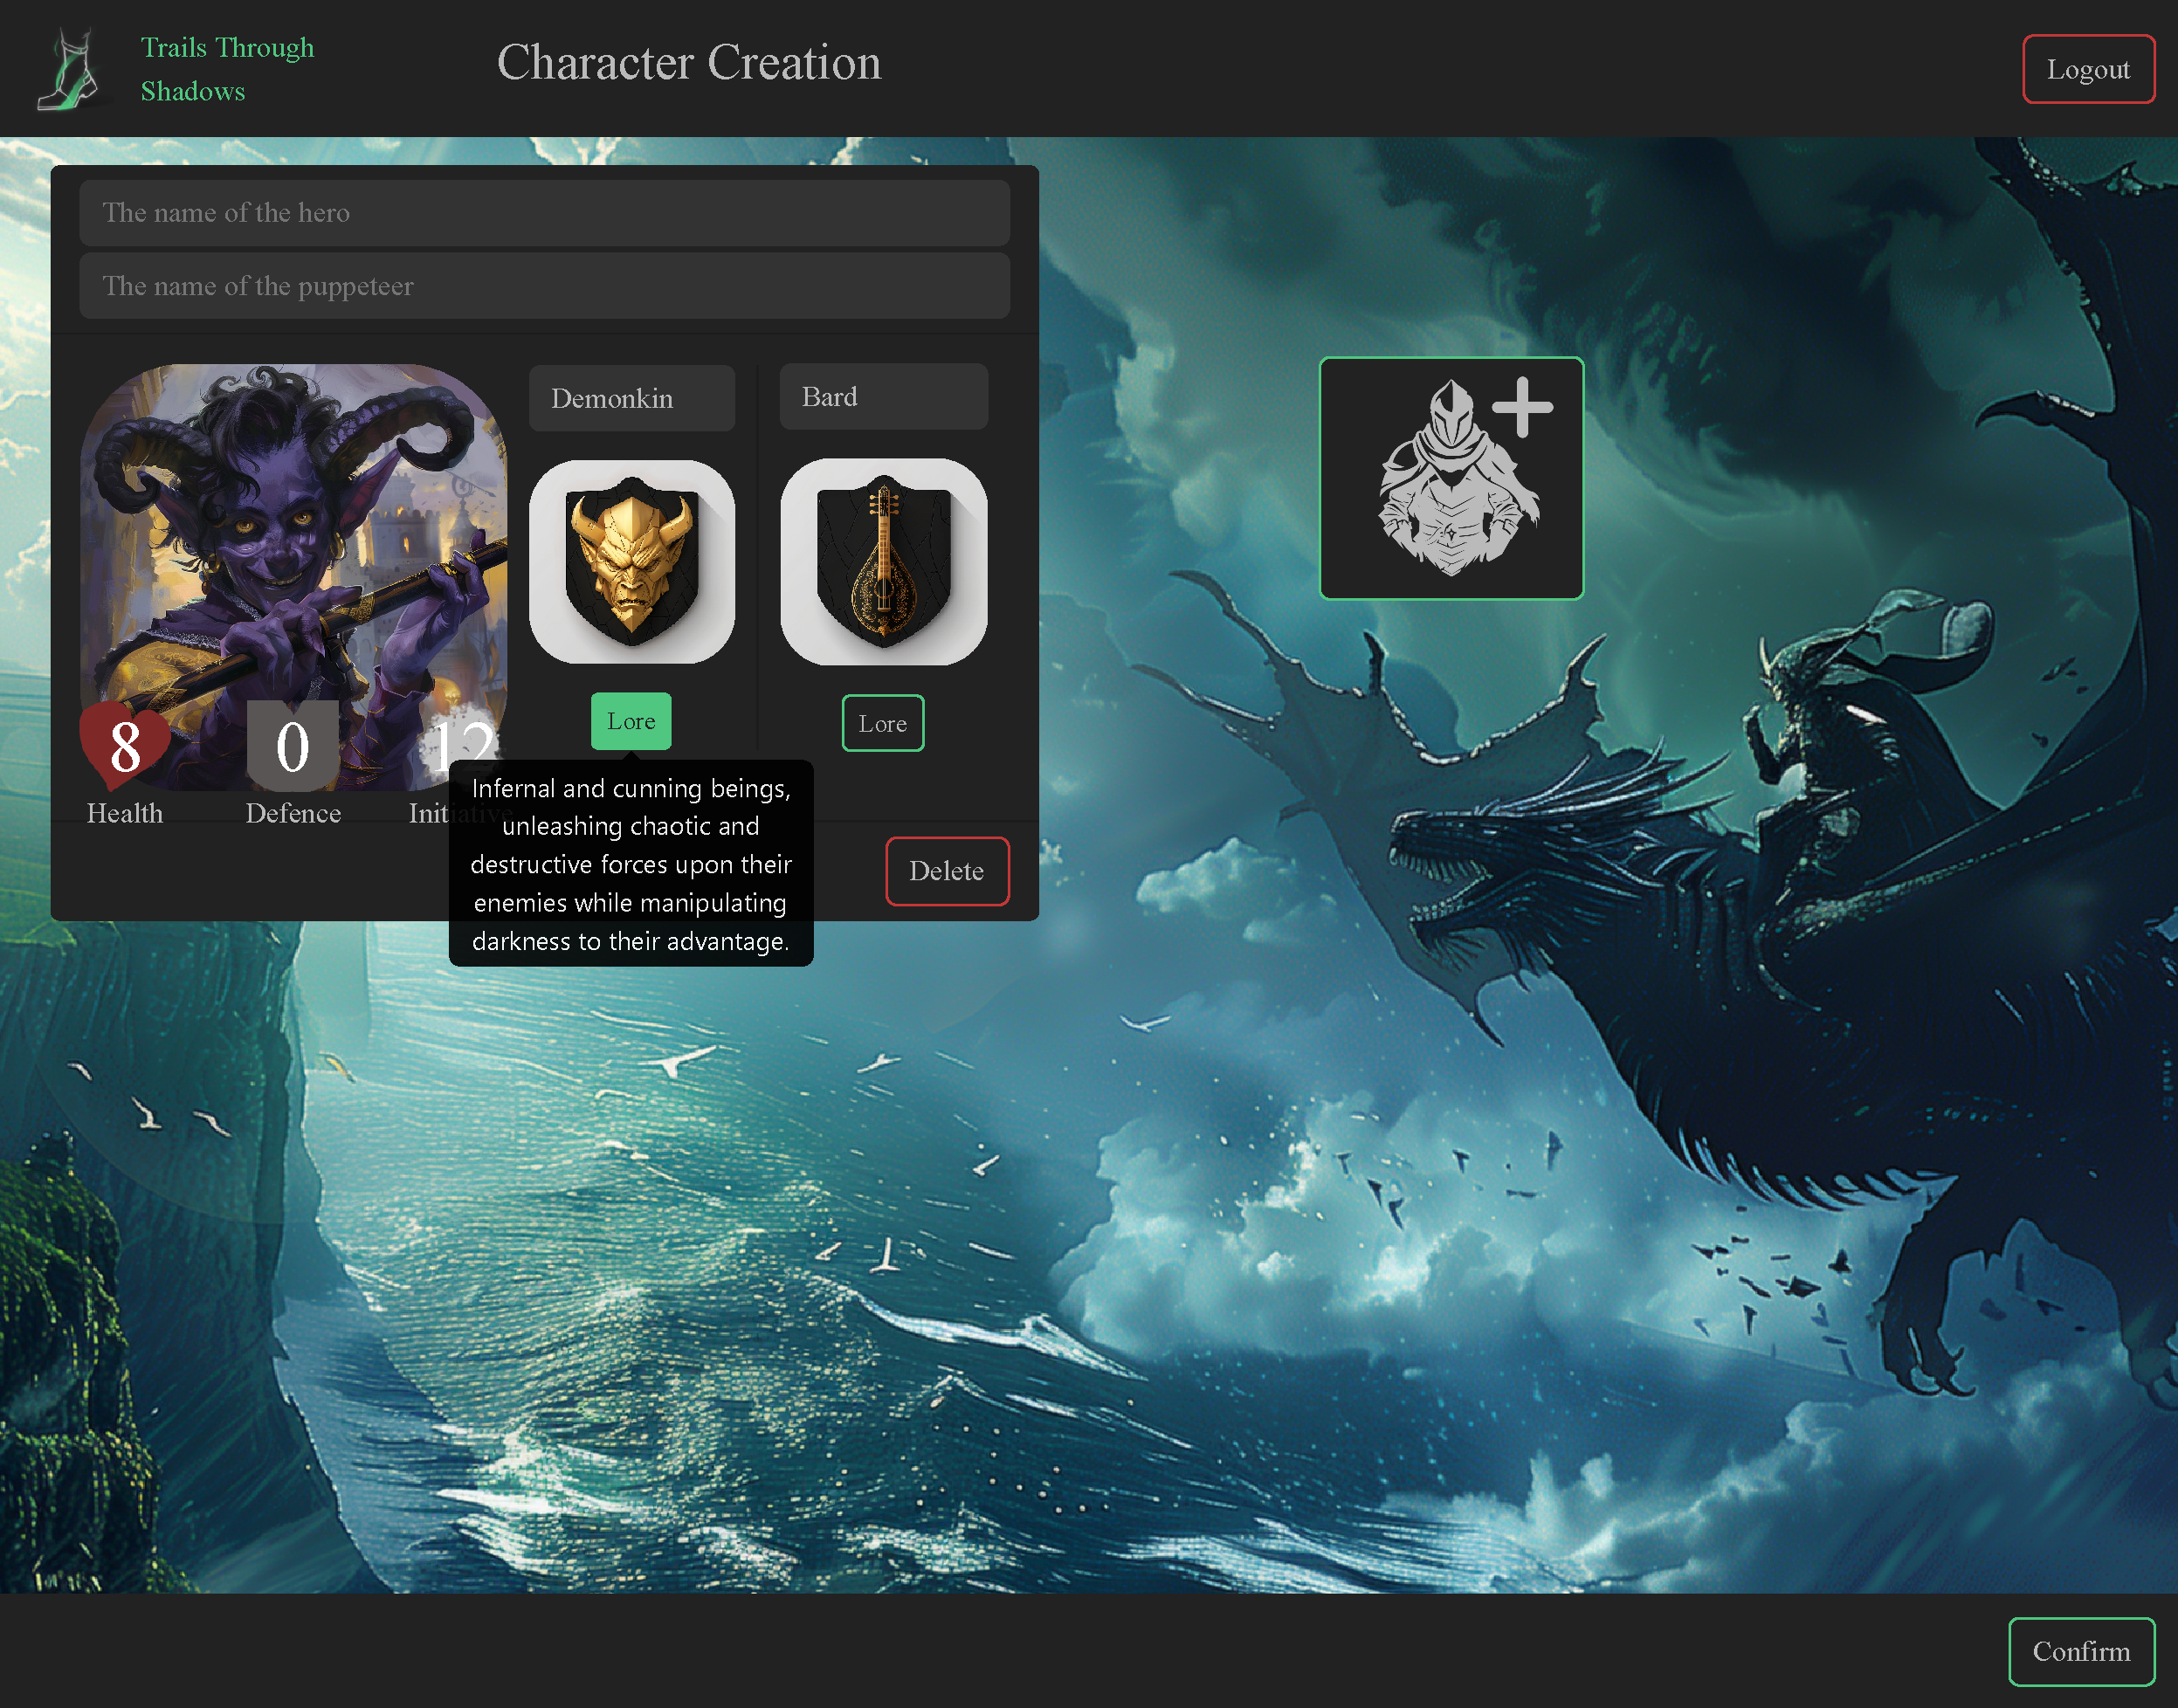
\includegraphics[width=.95\textwidth]{resources/figures/TTS-Charracter Creation.pdf}
  \caption{Snímek obrazovky komponenty vytvoření postav}
  \label{fig:pdf}
\end{figure}